\documentclass[12pt]{article}
\usepackage[utf8]{inputenc}

\usepackage{lmodern}

\usepackage{enumitem}
\usepackage[margin=2cm]{geometry}

\usepackage{amsmath, amsfonts, amssymb}
\usepackage{graphicx}
%\usepackage{subfigure}
\usepackage{tikz}
\usepackage{pgfplots}
\usepackage{multicol}

\usepackage{comment}
\usepackage{url}
\usepackage{calc}
\usepackage{subcaption}
\usepackage[indent=0pt]{parskip}
\usepackage{animate}

\usepackage{array}
\usepackage{blkarray,booktabs, bigstrut}
\usepackage{bigints}

\pgfplotsset{compat=1.16}

% MATH commands
\newcommand{\ga}{\left\langle}
\newcommand{\da}{\right\rangle}
\newcommand{\oa}{\left\lbrace}
\newcommand{\fa}{\right\rbrace}
\newcommand{\oc}{\left[}
\newcommand{\fc}{\right]}
\newcommand{\op}{\left(}
\newcommand{\fp}{\right)}

\newcommand{\bi}{\mathbf{i}}
\newcommand{\bj}{\mathbf{j}}
\newcommand{\bk}{\mathbf{k}}
\newcommand{\bF}{\mathbf{F}}

\newcommand{\mR}{\mathbb{R}}

\newcommand{\ra}{\rightarrow}
\newcommand{\Ra}{\Rightarrow}

\newcommand{\sech}{\mathrm{sech}\,}
\newcommand{\csch}{\mathrm{csch}\,}
\newcommand{\curl}{\mathrm{curl}\,}
\newcommand{\dive}{\mathrm{div}\,}

\newcommand{\ve}{\varepsilon}
\newcommand{\spc}{\vspace*{0.5cm}}

\DeclareMathOperator{\Ran}{Ran}
\DeclareMathOperator{\Dom}{Dom}

\newcommand{\exo}[1]{\noindent\textcolor{red}{\fbox{\textbf{Problem {#1}}}\hrulefill}\\}
\newcommand{\qu}[4]{\noindent\textcolor{#4}{\fbox{\textbf{Section {#1} | Problem {#2}}} \hrulefill{{\fbox{\textbf{{#3} Points}}}}\\}}

\newcommand{\semester}{Spring 2023}

\newcommand{\CVup}{%

\begin{tikzpicture}
\draw[black, <->, >=latex] (-0.33, 0.5) .. controls (-0.125, 0) and (0.125, 0) .. (0.33, 0.5);
\end{tikzpicture}}

\newcommand{\CVupInc}{%
\begin{tikzpicture}
\draw[black, ->, >=latex] (0,0) .. controls (0.2, 0) and (0.4, 0.2) .. (0.5, 0.5);
\end{tikzpicture}}

\newcommand{\CVupDec}{%
\begin{tikzpicture}[rotate=270]
\draw[black, ->, >=latex] (0,0) .. controls (0.2, 0) and (0.4, 0.2) .. (0.5, 0.5);
\end{tikzpicture}}

\newcommand{\CVdown}{%
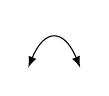
\begin{tikzpicture}
\draw[black, <->, >=latex] (-0.33, -0.5) .. controls (-0.125, 0) and (0.125, 0) .. (0.33, -0.5);
\end{tikzpicture}}

\newcommand{\CVdownInc}{%
\begin{tikzpicture}
\draw[black, ->, >=latex] (-0.5, -0.5) .. controls (-0.5, -0.3) and (-0.5, -0.1) .. (0,0);
\end{tikzpicture}}

\newcommand{\CVdownDec}{%
\begin{tikzpicture}[rotate=-90]
\draw[black, ->, >=latex] (-0.5, -0.5) .. controls (-0.5, -0.3) and (-0.5, -0.1) .. (0,0);
\end{tikzpicture}}

\begin{document}
	\noindent \hrulefill \\
	MATH-241 \hfill Pierre-Olivier Paris{\'e}\\
	Solutions Section 3-5 \hfill \semester \\\vspace*{-1cm}
	
	\noindent\hrulefill
	
	\spc
	
	\exo{10}
	\\
	
	Let $f(x) = \frac{x^2 + 5x}{25 - x^2}$.
	
	\begin{enumerate}[label=\textbf{\Alph*.}]
	\item We have $25 - x^2 = 0$ when $x^2 = 25$. So the denominator is $0$ when $x = \pm 5$. The domain is then $(-\infty , -5) \cup (-5, 5) \cup (5, \infty )$.
	\item For $x = 0$, we find $f(0) = 0$. Also, we have $f(x) = 0$ when $x^2 + 5x = 0$. So the $x$-intercept is $x = 0$.
	\item No symmetry, unfortunately.
	\item We first find the HAs and then the VAs.
		\begin{enumerate}[label=\textbf{(\Roman*)}]
		\item We first rewrite the function as followed:
			\begin{align*}
			f(x) = \frac{x^2 (1 + 5/x)}{x^2(25/x^2 - 1)} = \frac{1 + 5/x}{25/x - 1} .
			\end{align*}
		We can now see that
			\begin{align*}
			\lim_{x \ra \infty} f(x) = \lim_{x \ra \infty} \frac{1 + 5/x}{25/x - 1} = \frac{1}{-1} = -1
			\end{align*}
		and
			\begin{align*}
			\lim_{x \ra -\infty} f(x) = \lim_{x \ra -\infty} \frac{1 + 5/x}{25/x - 1} = \frac{1}{-1} = -1 .
			\end{align*}
		Therefore, $y = -1$ is a HA for $x \ra \infty$ and $y = -1$ is a HA for $x \ra -\infty$.
		\item We have $25-x^2 = (5-x)(5 + x)$ and $x^2 + 5x = x (x + 5)$. Therefore, the expression of the function becomes
			\begin{align*}
			f(x) = \frac{x (x + 5)}{(5 - x) (5 + x)} .
			\end{align*}
		Recall that we might have some problems at $x = -5$ and $x = 5$ because of the division by zero.
		
		 We first have
			\begin{align*}
			\lim_{x \ra -5} f(x) = \lim_{x \ra -5} \frac{x}{5 - x} = \frac{-5}{5 - (-5)} = -\frac{1}{2}
			\end{align*}
		and therefore there is no VA at $x = -5$. 
		
		Let's now examine the other possible problem at $x = 5$. We have
			\begin{align*}
			\lim_{x \ra 5^-} f(x) = \lim_{x \ra 5^-} \frac{x}{5 - x} = \frac{5}{0^+} = \infty
			\end{align*}
		and
			\begin{align*}
			\lim_{x \ra 5^+} f(x) = \lim_{x \ra 5^+} \frac{x}{5 - x} = \frac{5}{0^-} = -\infty .
			\end{align*}
		Therefore, we have a VA at $x = 5$.
		\end{enumerate}
	\item The derivative of the function is
		\begin{align*}
		f'(x) = \frac{5}{(x - 5)^2} .
		\end{align*}
	There is one critical number, which is $x = 5$ because the derivative does not exist there.
	
	The second derivative of the function is
		\begin{align*}
		f''(x) = -\frac{10}{(x - 5)^3} .
		\end{align*}
	There is one possible inflection point which is $x = 5$ because the second derivative does not exist there.
	\item We will now construct the table
		\begin{enumerate}
		\item Recall that $x = 5$ is a critical number. The sign of the derivative does not change because $(x - 5)^2 \geq 0$. Therefore, $f'(x) > 0$ when $x \neq 5$ and the function is increasing there.
		\item We have only one possible inflection point, at $x = 5$. When $x < 5$, then $x - 5 < 0$, so that $(x - 5)^3 < 0$. Therefore, because of the multiplication by $-10$, we obtain that $f''(x) > 0$. When $x > 5$, then $x - 5 > 0$ and $(x - 5)^3 > 0$. Therefore, we get that $f''(x) < 0$. 
		\renewcommand{\arraystretch}{1.5}
		\begin{center}
		\begin{tabular}{c||c|c|c|c|c}
		Derivatives & \phantom{22} $x < $ \phantom{22} & $-5$ & \phantom{22} $< x < $ \phantom{22} & $5$ & \phantom{22} $< x$ \phantom{22} \\\hline
		$f'(x)$ & $+$ &  & $+$ & $\nexists$ & $+$ \\
		$f''(x)$ & $+$ &  & $+$ & $\nexists$ & $-$ \\\hline
		$f(x)$ & \CVupInc & DNE & \CVupInc & VA & \CVdownInc
		\end{tabular}
		\end{center}
	\item We now see from the table that
		\begin{itemize}
		\item There is no maximum at $x = 5$.
		\item There is an inflection point at $x = 5$.
		\end{itemize}
		\end{enumerate}
	\item We can know sketch the graph of the function (see next page).
		\begin{center}
		\centering
		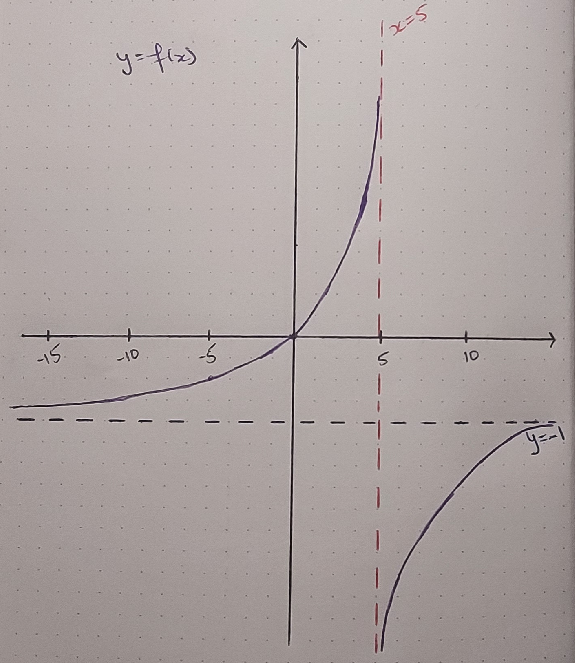
\includegraphics[scale=0.5]{no10.png}
		\end{center}
	\end{enumerate}
	
	\phantom{2}
	
	\newpage
	
	\exo{20}
	\\
	Let $f(x) = \frac{x^3}{x - 2}$.
	
	\begin{enumerate}[label=\textbf{\Alph*.}]
	\item We see that $x - 2 = 0$ when $x = 2$. Therefore the domain is $(-\infty , 2) \cup (2 , \infty )$.
	\item The $y$-intercept is $f(0) = 0$. The $x$-intercept is the values of $x$ giving $f(x) = 0$. The only $x$-intercept is then $x =0$.
	\item There is no symmetry.
	\item We will first find the HAs and then the VAs.
		\begin{enumerate}[label=\textbf{(\Roman*)}]
		\item We first see that
			\begin{align*}
			f(x) = \frac{x x^2}{x (1 - 2/x)} = \frac{x^2}{1 - 2/x} .
			\end{align*}
		Since $\lim_{x \ra \infty} \frac{2}{x} = 0$ and $\lim_{x \ra \infty} x^2 = \infty$, we have
			\begin{align*}
			\lim_{x \ra \infty} f(x) = \frac{\lim_{x \ra \infty} x^2}{\lim_{x \ra \infty} 1 - 2/x} = \frac{\infty}{1} = \infty .
			\end{align*}
		Similarly, we have $\lim_{x \ra -\infty} f(x) = \infty$. There is no HA.
		\item We have a problem when $x = 2$. Let's examine more closely this problem. We have
			\begin{align*}
			\lim_{x \ra 2^-} \frac{x^3}{x - 2} = \frac{(2^-)^3}{0^-} = \frac{8}{0^-} = -\infty .
			\end{align*}
		We also have
			\begin{align*}
			\lim_{x \ra 2^+} \frac{x^3}{x - 2} = \frac{8}{0^+} = \infty .
			\end{align*}
		There is a VA at $x = 2$.
		\end{enumerate}
	\item The derivative of $f(x)$ is
		\begin{align*}
		f'(x) = \frac{3x^2 (x - 2) - x^3}{(x - 2)^2} = \frac{2x^2(x - 3)}{(x - 2)^2}
		\end{align*}
	We find the critical numbers. The derivative does not exist when $x - 2 = 0$, so when $x = 2$. The derivative is $0$ if
		\begin{align*}
		\frac{2x^2(x - 3)}{(x - 2)^2} = 0 \iff 2x^2 (x - 3) = 0 \iff x = 0 \text{ or } x = 3 .
		\end{align*}
	The second derivative of $f(x)$ is
		\begin{align*}
		f''(x) = \frac{2x (x^2 - 6x + 12)}{(x -2)^3} .
		\end{align*}
	It is zero when $x = 0$ or $x^2 - 6x + 12 = 0$. But the polynomial $x^2 - 6x + 12$ is never zero because its discrimant is 
		\begin{align*}
		b^2 - 4ac = 36 - 48 = -12 < 0 .
		\end{align*}
	The second derivative does not exist when $x = 2$. 
		
	\item We now construct the table.
	
		\begin{enumerate}[label=\textbf{(\Roman*)}]
		\item The critical numbers are $x =0$ and $x = 3$. Since $(x - 2)^2 \geq 0$ and $x^2 \geq 0$, the sign of the derivative is determined by the sign of the factor $(x - 3)$. So, when $x < 3$, we have $x - 3 < 0$ and therefore $f'(x) < 0$. When $x > 3$, we have $x - 3 > 0$ and therefore $f'(x) > 0$. We input this information in the table.
		\item The possible inflection points are $x = 0$ and $x = 2$. Since $x^2 - 6x + 12 \geq 0$, the sign of the second derivative is determined by the sign of $x$ and of $(x - 2)$. If $x < 0$, then $x - 2 < 0$ and therefore the overall sign is $f'' (x) > 0$. When $x > 0$ but $x < 2$, then $x - 2 < 0$ and the overall sign if $f''(x) < 0$. When $x > 2$, then $x > 0$ and $x - 2 > 0$ and therefore the overall sign is still $f'(x) > 0$. We input this in the table.
	\renewcommand{\arraystretch}{1.5}
	
	\begin{center}
	\begin{tabular}{c||c|c|c|c|c|c|c}
	Derivatives & \phantom{22} $x < $ \phantom{22} & $0$ & \phantom{22} $< x < $ \phantom{22} & $2$ & \phantom{22} $< x < $ \phantom{22} & $3$ & \phantom{22} $< x$ \phantom{22} \\\hline
	$f'(x)$ & $-$ & $0$ & $-$ & $\nexists$ & $-$ & $0$ & $+$
	\\
	$f''(x)$ & $+$ & $0$ & $-$ & $\nexists$ & $+$ &  & $+$ \\\hline
	$f(x)$ & \CVupDec &  & \CVdownDec  & VA & \CVupDec &  & \CVupInc
	\end{tabular}
	\end{center}
	\item We now see from the table that
		\begin{itemize}
		\item There is no maximum at $x = 0$ and $x = 2$ from the First derivative test.
		\item There is a local minimum at $x = 3$ from the First derivative test. We have $f(3) = 27$.
		\item There is an inflection point at $x = 0$ and $x = 2$. 
		\end{itemize}
	\end{enumerate}
	\item We are now ready to sketch the graph of the function.
		\begin{figure}[ht]
		\centering
		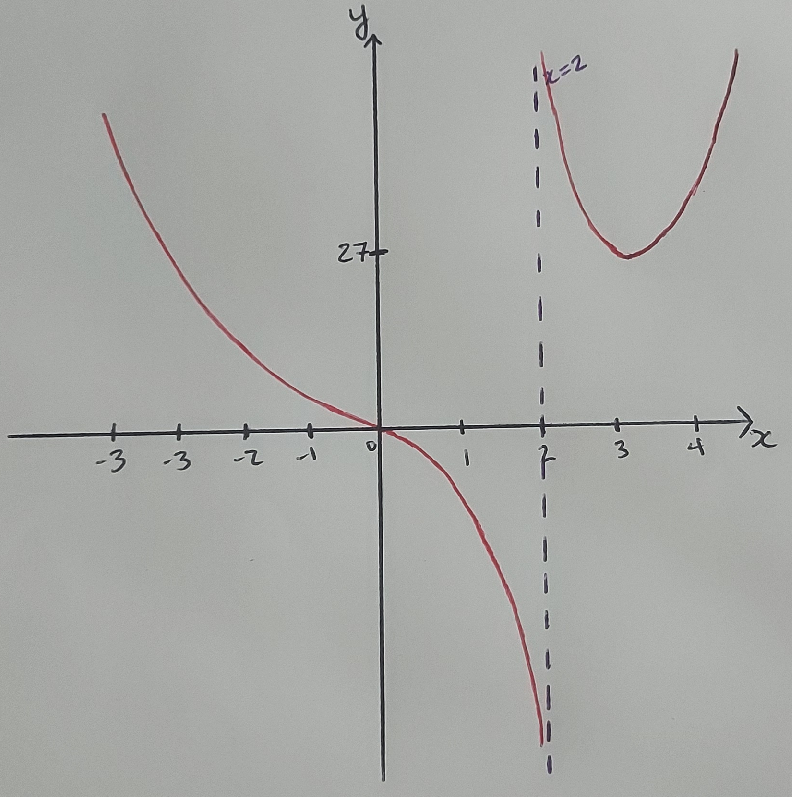
\includegraphics[scale=0.1842]{no20.png}
		\end{figure}
	\end{enumerate}
	
	
	
\end{document}
	